\documentclass[12]{article}

\usepackage{amsmath}
\usepackage{algorithm}
\usepackage[noend]{algpseudocode}
\usepackage{verbatim}
\usepackage[margin=1in]{geometry}
\usepackage{setspace}
\usepackage[utf8]{inputenc}
\usepackage[T1]{fontenc}
\usepackage{graphicx}
\usepackage{float}
\usepackage{wrapfig}


\makeatletter
\def\BState{\State\hskip-\ALG@thistlm}
\makeatother


\begin{document}
\onehalfspacing
\noindent
Jim Vargas\\
CS162 Programming Assignment 2\\
Algorithm and Flowchart
\begin{center}
Algorithm
\end{center}

	The program is intended to function as a simple encryption procedure. Hereon, let all instances of 'message' refer to the message which is to be transmitted, let 'block' refer to the paragraph of text in which the message is encrypted into, and let 'seed' refer to the process by which the message is encrypted with the block. These topics will be further defined below.
	
%\begin{wrapfigure}{l}{0.5\textwidth}%[H]

\begin{figure}
Flowchart\\
\centering
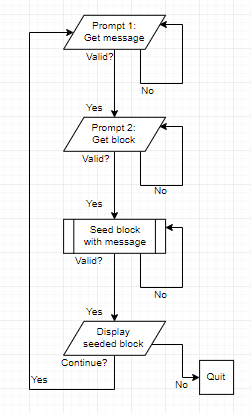
\includegraphics[scale=1]{flowchart.PNG}\\
\end{figure}

	Prompts:
\begin{enumerate}
\item First prompt:
	\begin{itemize}
	\item Greet user (as above).
	\item First, prompt for the message. This is to be a single sentence. 
	\item Second, get the message. Check to see if the input is valid, i.e., not blank, not too long, etc.
	\end{itemize}
\item Second prompt:
	\begin{itemize}
	\item Prompt for the block. This is to be a paragraph, i.e., multiple sentences.
	\item Get the block. Check to see if the input is valid, as above.
	\end{itemize}
\item Third prompt:
	\begin{itemize}
	\item Display encrypted message. Prompt the user to see if they wish to complete another cycle of the process.
	\end{itemize}
\end{enumerate}
Seeding:

	The first letter in each word in the block is replaced by a letter in the message. This replacement occurs sequentially; the first word in the block gets the first letter in the message, the second the second, etc. Additionally, the first letter of evey word in the message following the first (thus, not including the first), will be capitalized when replacing the corresponding letter in the block. The block's length, when returned having been seeded by the message, will be shortened to include only the necessary number of words to sufficienty seed the block.
	
   Here is an example:\\
message: "where does poop go"\\
unseeded block: "You may think this message is odd, but it is likely more original than this silly block."\\
seeded block: "wou hay ehink rhis eessage Ds odd, eut st Ps oikely oore Priginal Ghen ohis"\\
\\
Seeding Algorithm:
\begin{enumerate}
\item Loop through all characters in the block.
\item If the current character in the block is one which the preceding character was a 'space,' the current character is viable to be replaced.
\item For each character in the message, convert each viable character in the block with a message character, sequentially.
\item If the current character in the message is one which the preceding character was a 'space,' the current character will be capitalized in the block. That is, when a character in the block is replaced by a character in the message which followed a 'space,' it will be capitalized.
\end{enumerate}

	Here is a pseudo-code example of this algorithm.
\begin{algorithm}
\caption{Seeding Algorithm}\label{euclid}
\begin{algorithmic}
\Procedure{seed}{}
\State \bf{given:} \normalfont{message}
\State \bf{given:} \normalfont{block}
\State \bf{new data (\normalfont{List} \bf{of} \normalfont{Integers}\bf{):}} \normalfont{viablePositions}
\For {$each\,\,\,character\,\,\,in$ \normalfont{block}}
	\If {$current\,\,\,character\,\,\,position-1$ \bf{is} $\,\,\,a\,\,\,'space'$ \bf{or} $current\,\,\,position\,\,\,is\,\,\,zero$}
		\State $add\,\,\,current\,\,\,position\,\,\,to$ \normalfont{viablePositions}.
	\EndIf
\EndFor
\For {$iterate\,\,\,length\,\,\,of$ \normalfont{viablePositions}}
	\If {$current\,\,\,character\,\,\,position-1$ \bf{in} \normalfont{message} \bf{is} $\,\,\,a\,\,\,'space'$}
		\State \normalfont{block} @ \normalfont{viablePosition} @ $current\,\,\,iteration\gets$ \bf{uppercase:}  \normalfont{message} @ $current\,\,\,iteration$
	\Else
		\State \normalfont{block} @ \normalfont{viablePosition} @ $current\,\,\,iteration\gets$ \normalfont{message} @ $current\,\,\,iteration$
	\EndIf
\EndFor
\EndProcedure
\end{algorithmic}
\end{algorithm}

	In the second \textbf{for} loop, the algorithm uses layered indexing, using the '@' symbol. Notice, if there aren't an equal or greater number of words in the block as there are characters in the message, then the length of $viablePositions$ defined in the algorithm shall not be of sufficient length to fully seed the block with every word.


\end{document}